% HCI Group Konstanz Seminar Template
% Version 1.1
%
% ATTENTION: This template was designed to fit the most common requirements for different types of reports (e.g., Seminar to the Project or Project Report). However, if you feel the need to add an extra component or layout feature please talk to your advisor. Please do not change anything on this template unless it is explicitly allowed or agreed with your advisor. However, it is allowed to add packages that do not alter the design/layout of this template.
%

\documentclass[10pt, paper=a4, parskip, oneside]{scrreprt}
\usepackage[T1]{fontenc}
\usepackage[utf8]{inputenc}
\usepackage{hciknseminar}
\usepackage[ngerman, english]{babel} % Spell checking (Using ngerman for german spell checking). The last language is the standard language for the document.
\addbibresource{bibliography.bib}

% =========== Title page ============
\title{Evaluating Gesture Based Teleportation Techniques For Virtual Environments} % Your title
\type{Master Thesis} % Seminar to the Bachelor/Master Project | Bachelor/Master Project Report
\author{Philip Oesterlin} % Your name
\studentno{01/993546} % Your student number
\group{Human-Computer Interaction} % Do not change this
\department{Computer and Information Science} % Do not change this
\advisor{Jonathan Wieland} % Your advisor
\reviewer{Prof. Dr. Harald Reiterer} % Do not change this
\date{\the\day .~\monthname~\the\year}

% ============= Abstract =============
\abstract{
This is your abstract.
}

% ============= Document =============
\begin{document}
% Title page
\maketitle
% Abstract
\makeabstract
% Table of contents
\tableofcontents
\addcontentsline{toc}{chapter}{Contents} % Add contents to table of contents
% List of Figures
\listoffigures
\addcontentsline{toc}{chapter}{\listfigurename} % Add list of figures to table of contents
% List of Tables
\listoftables
\addcontentsline{toc}{chapter}{\listtablename} % Add list of tables to table of contents
% Prepare chapters
\clearpage
\setcounter{romanPages}{\value{page}} % Update variable for roman pages
\pagenumbering{arabic} % Turn on page numbering again

% ============= Chapters =============

\chapter{Introduction}
% 
\chapter{Introduction}
The world of virtual reality (VR) is getting increasingly diverse. All kinds of tools and games are built, pushing the boundary of what is possible to create with current technologies. The computing hardware is also getting more powerful and more consumer-friendly. Standalone headsets that do not require a powerful computer linked over a cable are cheaper and can even be more immersive since the user does not has to keep track of the cable. The next step on the path of simplifying the experience could be to make it possible to use VR without controllers. They will still have their place for applications that require very acuate tracking, lots of different types of inputs or where it makes sense to hold something like a gun or paintbrush. Many experiences do not require this, however. Especially for applications and tools used to collaborate, enabling users to enhance their communication with gestures might be helpful. Use-cases like this are where hand-tracking will allow the implementation of immersive, natural interfaces. This can allow anybody to just put the headset on and start interacting with the virtual world without first being told how to grab something or how to activate a button, as shown in figure \ref{fig:example}. However, as stated before, the interactions do have limitations in terms of accuracy and their number of inputs and are a challenge to get right. Users will first apply the mental model built during decades of experience using their hands in the real world. Differences between the real and the virtual world might therefore make the experience less immersive than if the user were using a controller where there is no previous knowledge. This raises the question of what to do if the virtual world allows users to do more with their hands than in the real world. 

\begin{figure}[!ht]
    \centering
    \includegraphics[width=\textwidth]{figures/examplegestures.png}
    \caption{Example of users interacting with objects in VR using hand-tracking. \cite{Han}}
    \label{fig:example}
\end{figure}


One simple way where VR technology can expand on what is possible in the real world is scale. The area a user is physically able to explore and walk around comfortably is limited. For most casual users of VR, that might be the size of their living room. In VR, this is not a limitation. There, a user can be given the ability to fly, teleport or use any number of so-called locomotion techniques to increase their level of comfort and allow them to go wherever they want. While not completely understood, the disconnect between the real world's movement and VR is likely one source of motion sickness. This makes locomotion a necessary mechanic to implement in large scale VR experiences and a very divisive one since it can impact the users' immersion and level of comfort a lot. VR experiences only offering continuous locomotion can, for some users that are more prone to get motion sick, only be usable for a few minutes, only with a limited field of view or not useable at all. On the other hand, users that are used to continuous navigation do not get motion sick as quickly or even at all report being frustrated by having to use another, less immersive locomotion mechanic that might get in the way a lot more. So while teleportation based locomotion is not needed for everyone, it allows most people to at least use large scale VR experiences comfortably without getting sick. This makes it the first and sometimes only mechanic that is implemented, and so it should be as well understood and implemented as possible. Especially when in combination with hand-tracking and gesture-based teleportation, there is only minimal research done so far.

This work expands the previously done research on how locomotion or, more specifically, teleportation should work using hand-tracking. Teleportation is the most popular form of locomotion in VR. When using controllers, locomotion is usually controlled using a joystick or button, and even though there are slight differences between each game, you can usually figure out quickly how to control it. Without controllers, there is no conventional way to control teleportation. The user can also not easily hit all the buttons until some feedback can lead them in the right direction. VR applications based on hand-tracking will, therefore, still have a learning curve for new users. If there is a standard way to use teleportation established, it should be based on research. 

% goal of the thesis

% maybe structure

% bilder





\chapter{Related Work}
% Introduction
Enabling simulated movement in virtual environments is not a new problem. 
The techniques that allow the user to move their viewpoint require special attention in regards to immersiveness, cybersickness, ergonomics and path integration, concepts explained in the following chapter.

% TODO: why sections are chosen


\section{Motion Sickness}\label{motion-sickness}

The phenomenon known today as motion sickness predates modern technology
by millennia and even Hippocrates wrote about it. The word ``nausea'',
the main symptom of motion sickness is also derived from the Greek word
for ship ``naus''. \cite{Golding} It is a very
unpleasant feeling and was even used as a legal punishment in the 19th
Century \cite{Reason}. The source of motion sickness is
well understood because there is a lot research from military agencies
since they had to transport a lot of soldiers by ship and needed them to
be healthy when they reached their destination
\cite{Johnson}. After the invention of the first flight
simulator, the term simulator sickness was coined. Simulator sickness is
a form of motion sickness that can occur when training pilots in
simulators \cite{Johnson}. With the rise of head mounted
displays and VR technology, motion sickness got another subcategory:
virtual reality sickness, also known as cybersickness. It is distinct
from simulator sickness because the symptoms are not as much related to
the Oculomotor system (for example eyestrain, blurred vision, etc) but
rather disorienting. The severity was found to be about 3 times greater
than simulator sickness. This might be because the VR systems are more
immersive than a flight simulator that relies on traditional displays
\cite{Stanney}.\\Because cybersickness and simulator
sickness are different, there needs to be a separate evaluation method
for the two phenomena. According to Stone et al. \cite{Stone} this is because the
weighted scale of the simulator sickness questionnaire does not
translate well to the VR environment. This is improved with a new
weighting scale proposed by Stone et al. \cite{Stone} but a new questionnaire
specifically created for cybersickness generates the best results.
However the simulator sickness questionnaire is often used in reached
anyway. This only has the benefit that the results are easy to compare
but there are significant tradeoffs in regards to accuracy.

\subsection{Cybersickness}\label{cybersickness}

As discussed before, cybersickness is a form of motion sickness. It can
result in a range of symptoms including nausea, vomiting,
disorientation, headaches and eye strain
\cite{LaViola}. This is a serious problem and needs to
be taken into account when developing VR systems.

% TODO: indent direct quote
The actual cause of cybersickness is not
known and the underlying physiological responses uncertain. According to Davis et al. \cite{Davis} The three
most prominent theories for the cause of cybersickness are poison
theory, postural instability theory and sensory conflict theory.

\begin{itemize}
\itemsep1pt\parskip0pt\parsep0pt
\item
  Poison theory: survival mechanism that induces vomiting and nausea to
  remove poison from the body if the brain detects sensory input like
  hallucinations.\\
\item
  Postural instability theory: a loss of postural control causes
  sickness\\
\item
  Sensory conflict theory: symptoms are created if there is a conflict
  between the vestibular and visual senses. For example if a user is not
  moving but their avatar in VR is.
\end{itemize}

Unfortunately all three theories have low predictive power and fail to
explain some key aspects of cybersickness~\cite{Davis}.

One way to reduce cybersickness is to break the optical flow the user
perceives using different kinds of techniques
\cite{Bhandari}. Optical flow is a phenomenon that
allows an observer to gather information about the motion of objects and
give the observer a sense of presence \cite{Gibson}.

\section{Locomotion in VR}\label{locomotion-in-vr}
% TODO: cite
The ability to move the players avatar in the virtual environment is
called locomotion. It is required for many applications or games that
take place on a larger scale. Without locomotion techniques VR would be
very inaccessible. A user would need a giant tracking space, which is
not possible in most homes and also the technology to track the users
headset would have to work over that amount of space. Locomotion is also
needed even if you could walk everywhere in your space, since it can
also be a convenience or accessibility feature in combination with a
seated experience. Getting the locomotion mechanics just right, will
also improve other interactions and user satisfaction in general. Moving
to a different virtual altitude would also not be possible without some
technique that can simulate the player walking up stairs. Otherwise
every user would have to have stairs in their tracked space. The
implementations of locomotion techniques can be very divers and so there
is a wide range of categorizations schemes.

Luca et al. \cite{Luca} collected 109 different locomotion techniques from academic
sources, social media and popular VR games. The result is a public
database of methods that can be filtered and compared. Some of the
methods are in a preliminary state and not fully implemented or
evaluated but in general the database is a great resource. There are only 8 results for hand-tracking
are some of them are falsely categorized.

\subsection{Locomotion using controllers}\label{locomotion-using-controllers}

Boletsis et al. \cite{Boletsis} categorized the four
prevalent locomotion techniques into:

\begin{itemize}
\itemsep1pt\parskip0pt\parsep0pt
\item
  Room-scale-based: uses physical movement, translates movement from the
  read world one to one into VR. continuos movement, unlimited range.\\
\item
  Motion-based: uses physical movement for example swinging arms or
  walking in place. Continuos movement, unlimited range\\
\item
  Controller-based: The uses controller input like a joystick to move.
  Continuos movement, unlimited range.\\
\item
  Teleportation-based: the viewpoint is instantly moved to a new
  predefined location. Non-continuos, unlimited range
\end{itemize}

The room-scale-based techniques are limited to the size of the tracking
space so they are not flexible enough for a general use case. If the
task allows it, it should however be the preferred locomotion technique
because it results in the best immersion while also keeping
cybersickness to a minimum.

Controller-based techniques could be adapted into a hand-tracking
environment, the continuos nature of the movement, without some kind of
a physical representation of the movement performed by user however
would make it prone to create motion sickness.

Motion-based techniques are very dynamic because of their physical
nature. That makes them hard to track with current hand-tracking
technology. They also made users tired the fastest.

For those reasons the scope of this work will focus on only
teleportation-based techniques to give results that as widely useable as
possible and accessible to the most amount of people without inducing
cybersickness.

\subsubsection{Teleportation-based locomotion}\label{teleportation-based-locomotion}

Teleportation is one of the most used locomotion techniques. Each
implementation can be slightly different in the way it is integrated
into the virtual environment but the core mechanic allows the user to
move the viewpoint to points on the map using some ray casting system.
There is usually a limit to the teleport distance and sometimes the user
is only allowed to select predefined locations as targets. The technique
is categorized as non-continuos movement with unlimited range. Since not
only the xy coordinates of a target location can be chosen but also
points at different altitudes, the method has 3 degrees of freedom.

The research from Clifton et al. \cite{Clifton} shows that on average teleportation
causes less cybersickness than continuos navigation, however, there were
some people (38\%) that had the opposite reaction.
Clifton et al. conclude that there should always be multiple locomotion
methods to choose from. The researchers theorize that the cause of the
cybersickness might be that some people are more sensitive to the
immediate displacement used by teleportation-based locomotion. If the
participants experienced the virtual environment while sitting or
standing did not make a cause a meaningful change in the reported
effects, only that there seems to be slightly worse cybersickness from a
seated experience. 

However, teleportation is also not the perfect solution. 
The lack of optical flow between locations is great to minimize
cybersickness, but it also introduces limitations. 
Path integration, a process where the brain updates the current position
continuously using information from different senses. Visual, vestibular
and proprioceptive sensory input are continuously integrated and create
a rough estimate of the distance traveled. \cite{Bhandari}

Bhandari et al. \cite{Bhandari} found that this can be improved by allowing some optical
flow between teleport points without creating higher levels of
cybersickness. This can be achieved by using a technique the researchers
call ``Dash''. It translates the user at a constant velocity from the
current point to the target. This creates a short transition period that
takes a maximum of 1.1 seconds over a maximum distance of 11 meters in a
virtual environment at real world scale. Previous research indicates
that the duration and speed do not impact the resulting effect a lot
\cite{Bowman} but these values where picked after some
internal testing. Using this technique users where able to move back to
a starting point after teleporting away much more accurately without any
landmark or context clues. 

An interesting problem with teleportation-based locomotion is that is
was found to be the least immersive technique out of the four types
categorized by Boletsis et al. \cite{Boletsis}. This
could improve using hand-tracking because the users can use their own
hands and that might be more immersive for some people. % TODO: (maybe include in hypotheses)


\subsection{Locomotion using hand-tracking}\label{locomotion-using-hand-tracking}

Only a rather limited amount of research was done about locomotion using hand-tracking even though natural human-computer-interaction using gestures is not a new field of study. Schäfer et al. \cite{Schafer2021} conducted a study using very basic gestures. In their virtual environment the simplest gesture only requires the user to point a finger in a forward direction to produce a visual ray in the respective direction. If this ray intersects with a valid teleportation location, a little reticle appears on that point. This marks the teleportation target. If the user keeps their hand still for 1.5s the teleportation to the target location is performed. Schäfer et al. also implemented other variations on this gesture:

There are two ways to select a location:
\begin{itemize}
  \item point index finger to select a location, named the index method
  \item use the normal vector of the palm to select a locomotion, named the palm method
\end{itemize}

There are also two ways to confirm a target:
\begin{itemize}
  \item the user keeps their hand still for 1.5s
  \item the user uses a second hand to confirm the location. For this a method was implemented where the left hand can first rests in a neutral position while a target is selected with the right hand. To confirm the teleport location, the user performs a pointing gesture with the second hand while keeping the right hand on the target.
\end{itemize}

The results of a user study conducted by Schäfer et al. \cite{Schafer2021} show the method using a one-handed palm gesture achieved the highest user satisfaction ratings (90 of 100 possible points). However, there appear to be some problems with the implementation. The authors noticed that bimanual methods loose tracking more often so this might influence the immersion and user satisfaction results. Another tracking issue was also found with the index method. The noise in the tracking data appears to frustrate users when trying to select a target. The tracking issues make it seem like the one handed palm gesture was only preferred by users because users found the unreliable tracking frustrating. This is also confirmed by the NASA-TLX results. The users reported to be more frustrated with the methods influenced by the bimanual tracking issues and the index finger tracking noise. The method influenced by both types of issues got the worst score. 

\begin{figure}[hbt!]
  \centering
  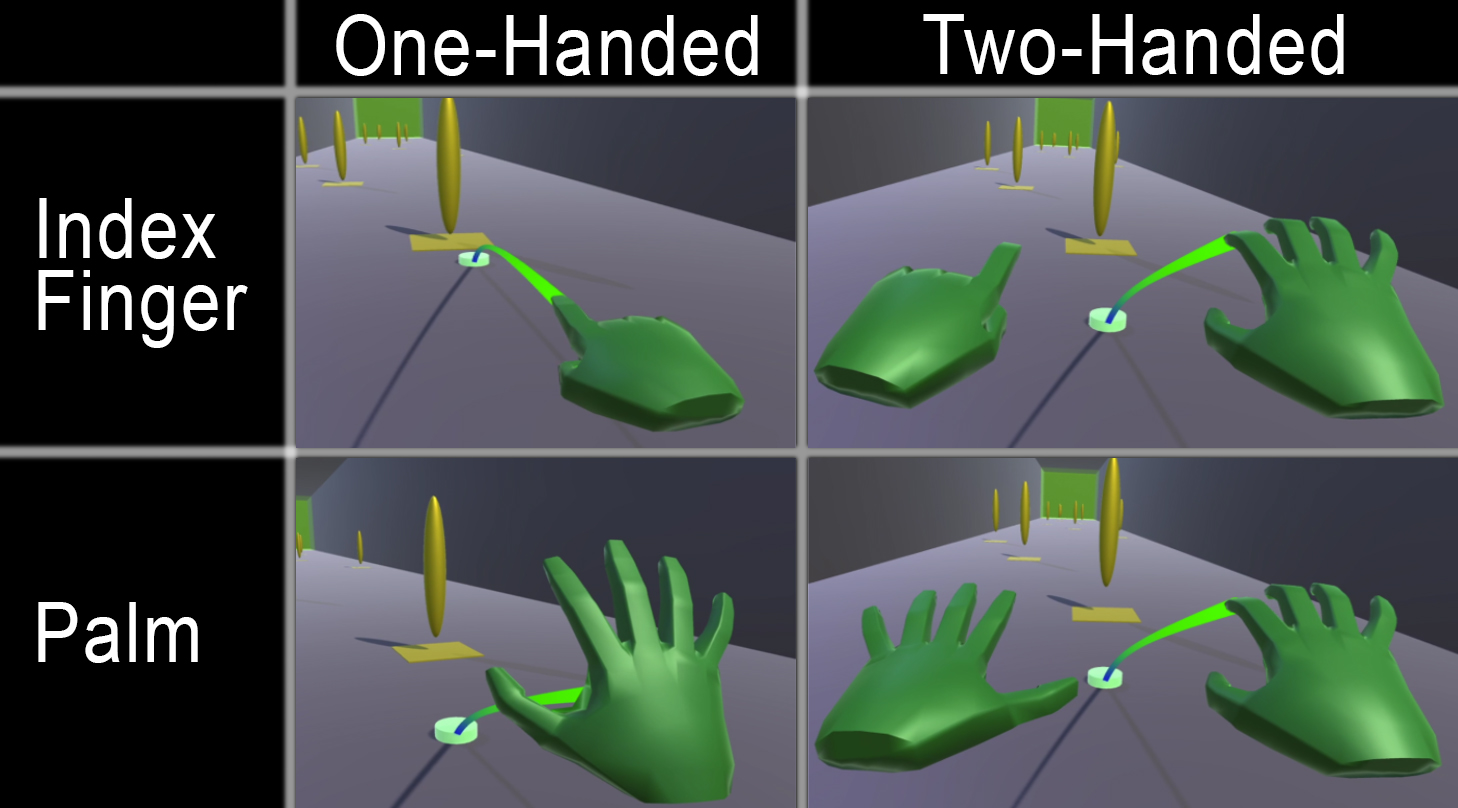
\includegraphics[width=\textwidth]{figures/1h vs 2h gesture study.jpg}
  \caption{Gesture types included in the study from Schäfer et al. \cite{Schafer2021}}
  \label{fig:1vs2}
\end{figure}

The one-handed palm method was the gesture that had the least amount of tracking issues since it was single handed and was not only using the index finger for target selection. This is result is surprising since the gesture violates multiple principles for a comfortable gesture detailed in \ref{ergonomics}. However, in a short study this might not influence the user satisfaction too much. The negative effects of uncomfortable gestures might not be noticeable after only using the gesture for the short duration of the study, so that the users are not experiencing the longer term effects. 

The one-handed palm method, the gesture with the highest usability score, also has other limitations. It would get even more uncomfortable when trying to teleport to some elevated targets. This would put a lot of strain on the wrist, which is one of the most problematic areas. The automatic confirmation of a target used also does not provide any feedback to the user like the bimanual methods do. Some of these issues can be improved on but it seems like the tracking is the most important issues to solve for now and that this is can only be solved using different gestures that enable more robust tracking with lest noise.

For traditional locomotion using controllers, the locomotion database from Luca et al. \cite{Luca} is a great resource. It includes solutions, that are user tested, established in the industry as well as more experimental ones. However, when filtering the locomotion database for techniques that are categorized to use hand-tracking only 8 results are presented.
The results that are relevant for this paper are:

\begin{itemize}
\item
  Hand Close: a gesture for continuos movement. Seems to have problems
  with cybersickness (25\% of study participants had to
  abort the 90 minute test). \cite{Huang}
\item
  Finger Run: two-handed gesture for continuos movement, the only
  resource is a video on a game development account that mostly posts fun
  prototyping ideas. \cite{Beauchamp}
\item
  Walking stick: a gesture instantiates a walking stick, that can be
  used to move the user in relation to the sticks touch point on the
  ground. This is only a preliminary database entry though and this is
  not a great solution for big distances or different altitudes. % TODO: cite
\end{itemize}

The categorizations seem to have some issues and so going through all
109 techniques, a small list of more gestures can be found that might work using gestures:

% TODO: integrate
\begin{itemize}
\itemsep1pt\parskip0pt\parsep0pt
\item
  World in miniature: manipulate player position on a miniature version of the environment
\item
  Cloudstep: small teleportation steps using a joystick
\item
  Dash Pointing: fast, continuos step in the direction of the controller with limited field of view
\end{itemize}

 % TODO: cite

Problems when trying to translate other methods into an environment without controllers:

\begin{itemize}
\item
  limited tracking space for hands: Controllers can still detect button
  presses and orientation changes if they are out of the tracking
  region, like behind the body. The hand-tracking system has no idea
  what the users hands are doing if they are out of view or obscuring
  each other.\\
\item
  limited accuracy: Hand-tracking is much less accurate with current
  technology. This might improve in the future though.\\
\item
  Hand-to-hand interaction is confusing the hand-tracking system\\
\end{itemize}

\section{Gestures}\label{gestures}

Emerging technologies enable new human-computer interaction techniques. Gestures are a core part of human communication so it only makes sense to adapt them for user interfaces. However, gestures are not new only the technology to be able to detect them is. There are also sources of information from other fields of research, like research on sign language, that can be of use to create gestures that are comfortable and intuitive.


\subsection{Gesture Detection}\label{gesture-detection}

The most accessible hand-tracking hardware for virtual reality today is
the Oculus Quest 2 VR headset. It has hand-tracking build in, which can
be accessed using the Oculus SDK in Unity. The exact technology the
Oculus Quest device uses is not known. However it can be speculated that
Oculus is using a variation of the research done by Han et al \cite{Han}. The
Oculus Quest only has monochrome cameras and only a very limited amount
of processing power, which correlates with the limitations addressed by
Han et al. \cite{Han}. Like the Oculus Quest, the
unnamed headset in the paper has 4 cameras. They are positioned on the
headsets corners, all facing in slightly different directions to cover a
120° area in front and below the headset. The areas the individual
cameras can see overlap in some places so that in the most important
areas the hands are visible for at least 2 up to 4 cameras. The
tracking system works by first detecting the hands in the camera streams
using a CNN architecture optimized for efficiency named DetNet. The
network can simultaneously localize and classify the hands which
combines two steps into one. Next, a network called KeyNet takes the the
cropped camera images and outputs 21 coordinates that match key points
of a human hand. The network architecture is optimized to reduce jitter
and consistency when moving between overlapping camera areas. This is
done using extrapolated points as an additional network input. The
output is suitable for basic interactions and certainty impressive for
real time processing on mobile hardware but there are definite
limitations. Since Hand-to-hand occlusions and interactions were not
part of the training set, the output has problems with complicated
poses.

% TODO: cite schäfer 3.3 capturing gestures

\subsection{Future Technology}\label{future-technology}

Current technology has some major limitations when tracking hands.
Hand-to-hand interactions, self-contact and occlusion come to mind.
Smith et al. \cite{Smith} created a system that takes in high resolution data from
124 cameras capturing uniformly lit hands. The images are turned into a
mesh so detailed its basically indistinguishable from the original
hands. The pose of two hands and even the texture is captured without
any artifacts. This process is very complex and it takes minutes to
render per frame so it will take some optimization until detailed hand
models like this could be included in a VR environment. However, this is
the direction that technology will go, even if it will take some time.
That means that even if hand-to-hand interaction is not able to be
reliably tracked currently, it could be in the future.

\subsection{Intuitive and comfortable gestures}\label{ergonomics}
For the design of a hand gesture vocabulary, the first consideration might be how well the gesture can be identified. However, gestures that are easily recognized may not be intuitive and easy to perform by the user. According to Stern at al. \cite{Stern2006} there are three factors that all should be maximized when choosing a gesture: intuitiveness, comfort and recognition accuracy.

Stern et al. define intuitiveness as the cognitive association between a command or intent and its physical gestural expression. Experiments that trying to find universal gestures for a virtual reality environment were also done by Pereira et al. \cite{Pereira2015}. The in the experiment 34 participants were asked to come up with gestures for common HCI tasks like. % TODO: sample
This resulted in over 1300 different gestures for 34 tasks. However, only 84 gestures were chosen by 3 or more subjects and some of them for different tasks. Expecting the user to intuitively guess the same gesture that the developers of the virtual environment intended therefore seems unrealistic. Constructing a gesture that requires no introduction or tutorial is therefore also not the goal of this paper.

The research of Ardito et al. \cite{Ardito2014} also supports this. They compare trying to design universal gestures to problems that arose with visual languages in the past. They predict that trying to use the same gesture vocabulary over a range of applications and devices is likely to fail. 


As a measure for comfort, Kölsch et al. propose a method that distinguishes between a pose of some joint or body part and the user compensating using other joints to relieve strain. A compensation for a pose that requires the users head to be tilted onto its side might be to keep the head upright relative to the body but bend the torso to the side. To find the optimal comfort zone of a posture, Kölsch et al. \cite{Koelsch} measure how users compensate or if they execute the pose without compensating. 

There are also other methods that rely on biomechanical models and physics simulations to measure how comfortable a gesture is but they are prone to errors \cite{Stern2006}.

Another source of knowledge to source information from regarding gestures are sign language interpreters. They might spend more than 20 h per week signing, however, they also often suffer from hand pain and fatigue while gesturing for long sessions. This would also be a risk for prolonged sessions in virtual reality that is using hand-tracking gestures. Rempel et al. conducted a study with experienced sign language interpreters to find the discomfort level associated with signing selected hand postures, motions and characters \cite{Rempel2014}. 

Rempel et al. \cite{Rempel2014} collected findings and summarized:
\begin{itemize}
  \item Hands should be near the midline of the body and not further apart than the shoulders. They should be near the height of the elbows and close to the lower chest, so that the shoulder muscles are not tense. 
  \item Sustained elbow flexion of more than 90 degrees should be avoided.
  \item The most comfortable postures were between neutral and 45 degrees of pronation (palms rotated toward ground). Repeated full rotations to palm up (supination) or palm down (pronation) should be avoided.
  \item Gestures that included movement of the elbow or shoulder were more comfortable than gestures with just finger movements.
  \item The more comfortable gesture motions were up-down hand movements performed with motion at the elbows or side-to-side hand movements with motion at the shoulders. 
  \item the most comfortable hand gestures were with the wrists straight and the fingers slightly flexed or in a loose fist.
  \item The least comfortable gestures were those involving wrist flexion; discordant adjacent fingers; or fingers extended.
  \item The position of the thumb did not appear to have a large influence on comfort.
\end{itemize}



\section{Usage in Games}
In the games industry there are some examples of gesture based movement present. The gestures used are probably tested and evaluated internally but there is currently no information published how well they work statistically, if they are ergonomic or usable. That means that for now, they can only be compared on a basis of personal experience. 


\subsection{Vacation simulator}
Vacation simulator \cite{VacSimOculus} is a VR simulation game, the sequel to the popular game Job Simulator. Released in 2019 by Owlchemy Labs, it was updated in late 2020 to enable hand-tracking support \cite{VacSimBlog}. The game has a lot of intuitive mechanics that translate very well to hand-tracking, like its use of a physical backpack as a game menu. The teleportation system is very easy to control but comes with the limitations that the user can only teleport to large predefined areas. Therefore, the gesture does not need to be very accurate. The user only needs to "pull" the target closer using a gesture shown in \ref{fig:pull}. 

\begin{figure}[hbt!]
  \centering
  \includegraphics[width=\textwidth]{figures/vacsim.jpg}
  \caption{Selecting a target area and confirming teleportation in Vacation Simulator}
  \label{fig:pull}
\end{figure}

This works well for this use case, where the teleportation does not need to be accurate. During testing, this was never a problem and might have even be more intuitive than using a controller because its so easy to remember and control, whereas some unexperienced users sometimes seam to have problems with the activation of controller based teleportation using the joystick. 


\subsection{Elixir}
One of the first hand-tracking titles for the Oculus Quest was Elixir. A short demo game where a user is allowed to explore a magic chamber. The chamber could be explored using Room-scale-based movement if the user has a large enough play space, however there is also a teleportation system included. It works using a bimanual gesture. Both hands form a triangle using both thumbs and index fingers. This can be used to target a point on the floor. The teleport resolution is limited to a grid system on the floor. Once selected a tile on the floor lights up. To confirm the tile as the target location, the user pinches the respective thumbs and index fingers together. The viewpoint is the instantly moved to the new location.

\begin{figure}[hbt!]
  \centering
  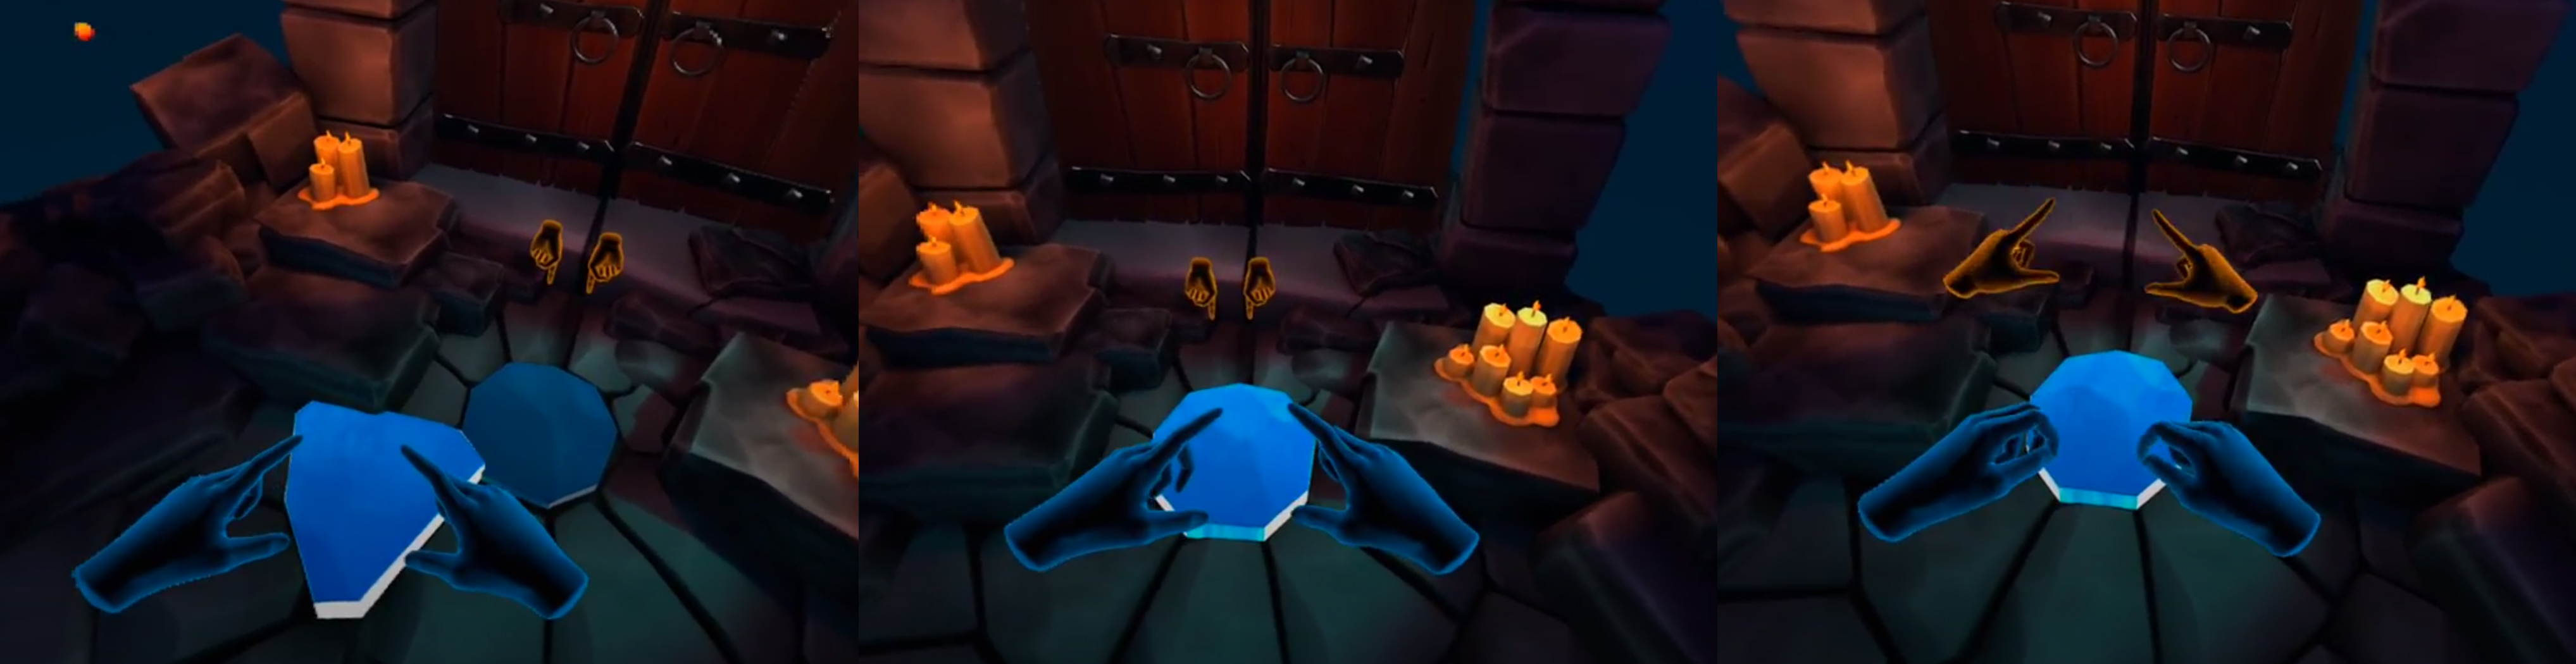
\includegraphics[width=\textwidth]{figures/elixir.jpg}
  \caption{Selecting a target and confirming teleportation in Elixir}
  \label{fig:elixir}
\end{figure}

The system does not allow the user to teleport to any point which is technically a limitation. However, in practice it makes the tracking more stable while sill allowing good control. Having a gesture to confirm makes the system feel controllable. 


\subsection{Waltz of the Wizard}
In the fantasy game Waltz of the Wizard \cite{WaWizOculus} by the Studio Aldin Dynamics \cite{Aladin}, the user can learn spells and have fun manipulating the environment. The game has been updated to support hand-tracking \cite{WaWizBlog}. This also includes an adaptation of the custom teleport system the game used in its original version called Telepath \cite{WaWizTelePath}. To move, the user draws a path on the floor. This path is broken up into sections. The system moves the users viewpoint from one point to the next, while dynamically adjusting the pause between the teleport steps. This allows the user to pick up objects while walking, or increase the walking speed by swinging arms. In contrast to the other systems, Telepath can be used to move to any point, without the limitations of the other systems. It does not require a grid system on the floor and is not limited to only specified teleport points.

\begin{figure}[hbt!]
  \centering
  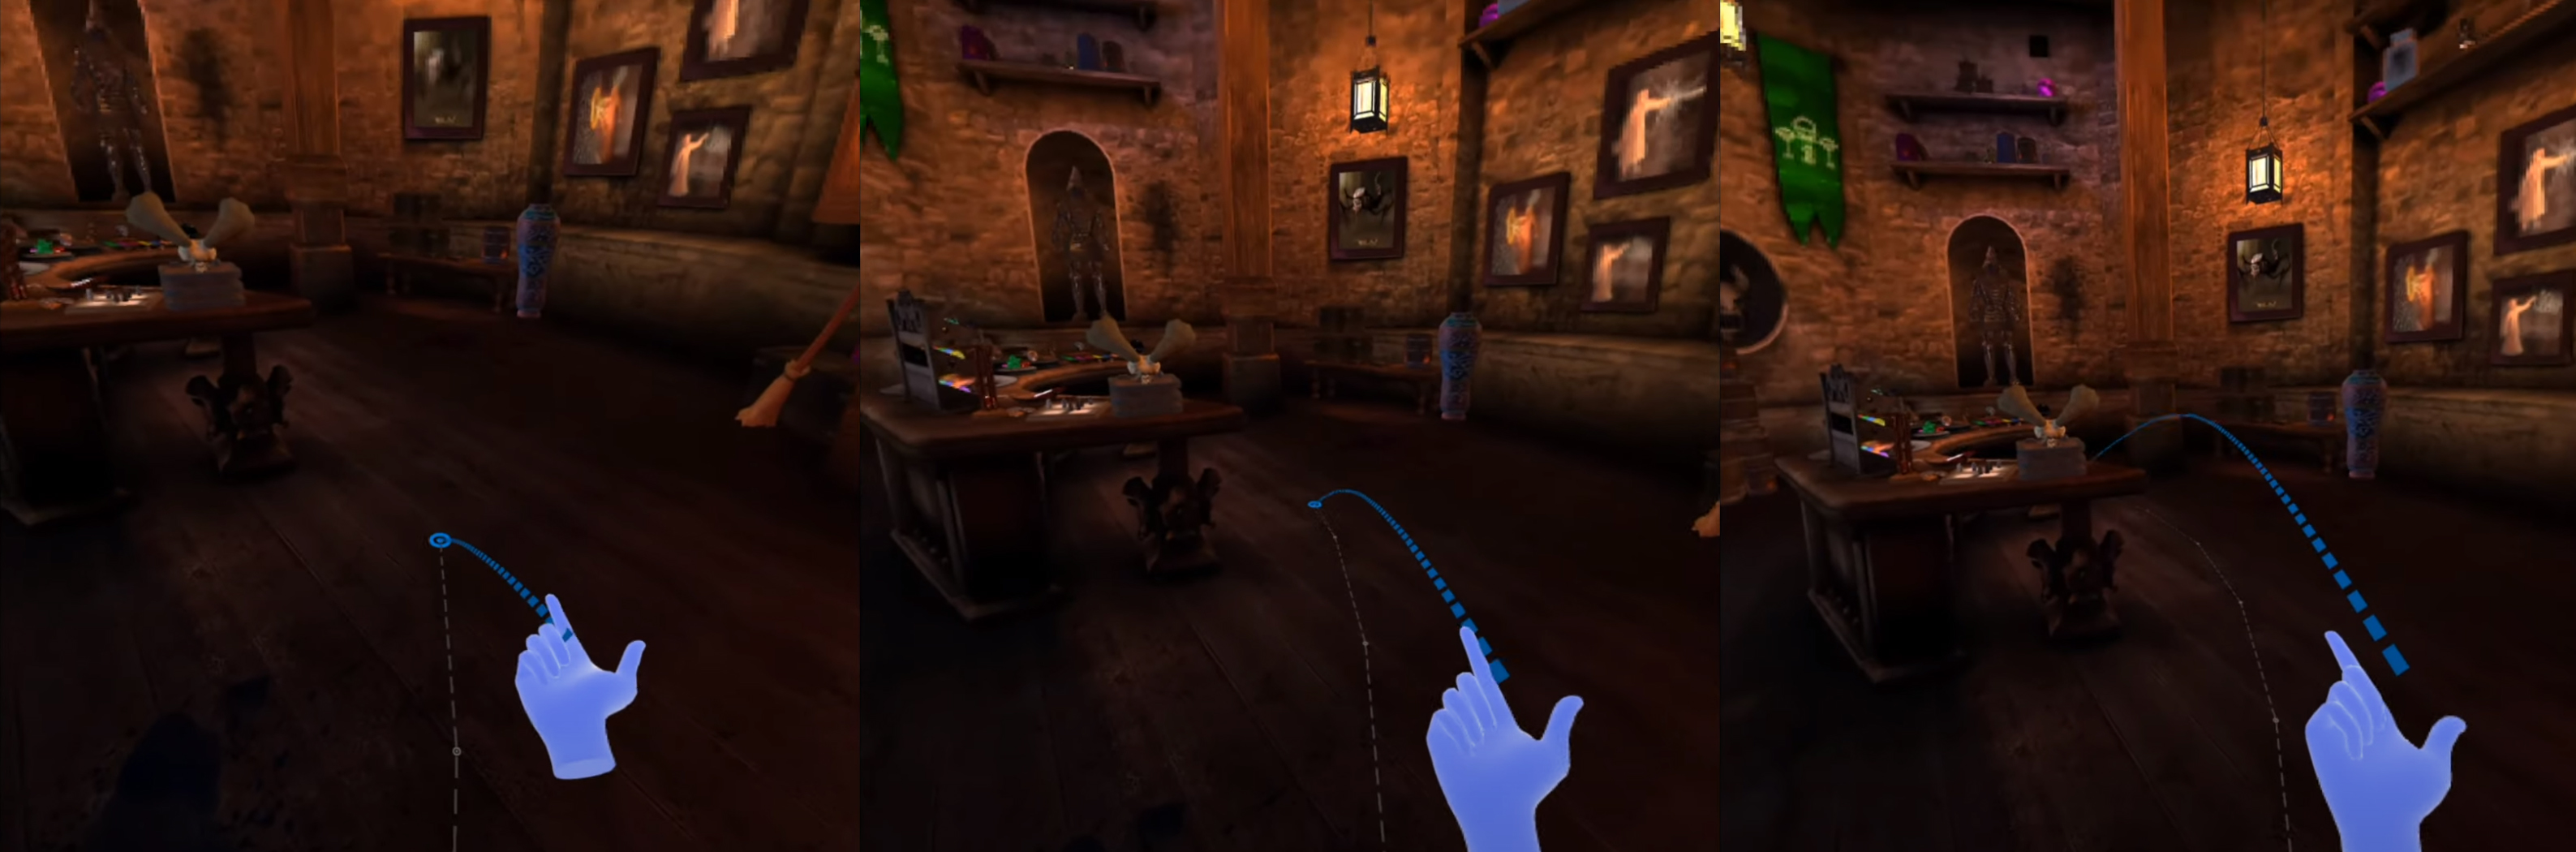
\includegraphics[width=\textwidth]{figures/waltz of the wizard - point.jpg}
  \caption{Telepath gesture: draw walking path using index finger}
  \label{fig:telepath}
\end{figure}

During testing, the Telepath system did not induce cybersickness even though the movement did required a short period of getting used to. The accuracy of the gesture recognition system left a lot to be desired however and the experience was frustrating at times. Ergonomics are also a point to criticize, size the gesture strains the hands quite uncomfortably even after only a short test of 20 minutes. Drawing a path still seams to be a promising idea and might enable high levels of immersion and allow the brain to perform path integration while not inducing cybersickness. Short bursts of quick movements have also been analysed by Bhandari et al. \cite{Bhandari}. It produced promising results regarding cybersickness and and path integration. 

\section{Study Designs}
For the comparative user study, it is helpful to look at methods used in the literature. 


The study designed by Bozgeyikli et al. \cite{bozgeyikli} compares 3 locomotion systems in the same environment. A gesture based point and teleport system, a walk in place system and a system using a joystick. The later two are continuos locomotion systems, while the first is a teleportation system. The environment was designed to be very basic to keep the focus on the locomotion. It includes 6 target points with a 0.6m radius placed on the ground. There are also 21 obstacle pillars scattered around in the environment. The task for the users is to move to a highlighted target, to wait for 3 seconds on the point and then move on to next point.

The independent variable in this study and all others described here, is the gesture tested. The dependent variables are the time to reach destination points, the number of collisions with the obstacles and the results of the usability survey. 
However collisions can only occur while using the two types of continuos locomotion. 



The study designed by Schäfer et al \cite{Schafer2021} also uses a primitive environment in the form of a long corridor to reduce the wow effect for first time users. The environment includes ten markers spaced out along the corridor. The participants task is to touch all the markers while traveling through the corridor. To explain the gestures an introduction is added to the study in form of a tutorial video.

In this case the dependent variables are the task completion time, the number of teleports, the number of times the tracking is lost and the results of a usability survey.


The study designed by Caggianese et al. \cite{Caggianese} uses a detailed, immersive environment as shown in \ref{fig:path}. It includes a very long path way of 343m with distractors along the way. The users task is to follow the path from start to end. 

The dependent variables in this case are efficiency and effectiveness of each gesture. Efficiency is derived from completion time. The effectiveness is derived from performed errors, locomotion interruptions and tracking errors. There are also five questionnaires (SSQ, SAM, SUS, SEQ, NASA-TLX) for each participant to fill out after each run.

\begin{figure}[hbt!]
  \centering
  \includegraphics[width=\textwidth]{figures/path-of-study.PNG}
  \caption{Caggianese et al. \cite{Caggianese} Task}
  \label{fig:path}
\end{figure}


The study designed by Bhandari et al. \cite{Bhandari} uses an extremely basic environment with only a ground plane and a sky above. This is so that the brain is not able to compute path integration from context clues. The users task is to move to a self-selected target point in the distance, to turn around and then to try to hit the start point again. A diagram is shown in \ref{fig:backAndForth}.

\begin{figure}[hbt!]
  \centering
  \includegraphics[width=\textwidth]{figures/back-and-forth.png}
  \caption{Bhandari et al. \cite{Bhandari} Task}
  \label{fig:backAndForth}
\end{figure}

In this case the dependent variable is how large the distance $a$ is. From this value it is derived how well the brain is able to grasp how far the traveled distance was and how repeatable the gesture is.

\section{Conclusion}
The research done so far has not produced a conclusive answer how to teleport using hand gestures. It is even disputed if such a solution is possible to find at all. The game industry has found some methods for different use cases and environments, there is however no way to compare them in a controlled environment, since they are each implemented in their respective games. The goal of this project is therefore, to create a test environment to compare methods from the literature and selected games in a standardized way. 


\chapter{Study Design}
% Introduction
The user study to compare teleportation techniques and to provide quantitative figures is detailed in the following chapter.


\section{Requirements}
This section explains the requirements set to evaluate the gesture.
For the study, the requirements have to be measurable. Therefor criteria for every requirement have to be set:

\begin{enumerate}
    \item The gesture can be recognized by the tracking system with a success rate of at least 90\%
    \item The system is efficient and effective to use
    \item No more than 20\% of users experience some cybersickness, no participant has to abort the test prematurely
    \item Even after extended use, the gesture does create strain in over 10\% of participants
    \item System has a SUS score of above 90.
    \item The user can get a sense of the distance they covered
    \item The system encourages walking in real life if possible and is not used to travel distances below 50cm
\end{enumerate}


\section{Study Setup}
The user study to compare the selected teleportation systems with respect to the different requirements has multiple sections:
\begin{itemize}
    \item Gesture Recognition Test
    \item Main Test:
    \begin{itemize}
        \item Usability
        \item Cybersickness
        \item Ergonomics
        \item Encourages walking
    \end{itemize}
    \item Path integration Test
\end{itemize}

\subsection{Gesture Recognition Rate}
To test the gesture detection algorithm 3 different people run a test where they form the gesture 20 times and record how often the algorithm is able to recognize the gesture.
The goal of this test is not to test tracking system of the Oculus Quest 2, but to test the algorithm used for gesture detection. The detection of the hands is not perfect and struggles in some scenarios and poses. For the study a environment with consistently good lighting is needed to improve the tracking conditions. 


\subsection{Efficiency and Effectiveness}
To test the efficiency and effectiveness of the systems, the participants have to teleport from a starting point to a goal point. During the task shown in \ref{fig:turret}, a gun turret shoots particles if the user is in sight and is standing still. The user is instructed not to let this happen. The environment is supposed to be somewhat stressful but has a strong incentive on teleportation accuracy. The task completion time as well as the number of particle hits will be measured. All methods have the same maximum teleportation distance and the spacing between the hideouts is adjusted so that a user can never skip a hideout without getting in the sight of the turret. The order of the different teleportation techniques will be randomized to minimize the learning effect. The teleportation mechanics are supposed to fade into the background as they should in a regular application. 

\begin{figure}[hbt!]
    \centering
    \includegraphics[height=\textwidth/2]{figures/turret study.png}
    \caption{Gun turret fires if it can see the user, user has to get to goal point, obstacles can hide user}
    \label{fig:turret}
\end{figure}


\subsection{Usability}
The main part of the study is an extended task in an immersive, magical VR environment.
The task is to collect different ingredients for a magic potion from all over the map. The teleportation system will be changed after each object was found and brought back to the starting point. Each teleportation system is active twice and in a random order to minimize the learning effect. The user will receive a short in-game tutorial each time the locomotion system is changed and a picture of the next object that should be found. The locomotion will then be done entirely using the gesture and the user will have to use it extensively. The usability will be evaluated using a questionnaire after the experience. 


\subsection{Cybersickness}
Cybersickness will be evaluated after the main experience using a questionnaire.


\subsection{Ergonomics}
Ergonomics are evaluated by the guidelines listed in \ref{ergonomics}. Additionally after the main study the participants will receive a questionnaire that can be evaluated into a score.


\subsection{Path integration}
In a very basic environment without peripheral reference points, a user should be able to move away from the origin point A to a point in the distance B. The participant is then instructed to turn around and move back as close as possible to the start point A. The distance from the users hit point A` to the target A is measured. This can be compared to the distances that physical movement and teleportation using controllers create in the same setup. The distance should be somewhere between two and six meters but chosen by the user. Each user completes the same procedure with all three methods one after the other but the order is randomized for every user to minimize the learning effect. This method is the same that Bhandari et al. \cite{Bhandari} use in their study.


\subsection{Encouraging Walking}
In the main study environment, the user should still use physical walking if possible. To test this, the traveled distances are recorded. The distribution can be analysed.







% =========== Bibliography ===========
\chapter*{References} % Set custom bibliography heading
\renewcommand{\thepage}{\roman{page}} % Use roman page numbers again
\setcounter{page}{\theromanPages} % Set the page counter
\addcontentsline{toc}{chapter}{References} % Add bibliography to table of contents
\defbibheading{bibempty}{} % Remove standard bibliography heading
\printbibliography[heading=bibempty] % Print bibliography and set the heading to the defined empty heading

\end{document}
